\documentclass[12pt,a4paper]{article}
\usepackage[utf8]{inputenc}
\usepackage[T1]{fontenc}


\renewcommand{\baselinestretch}{1}

\setlength{\hoffset}{-18pt}         
\setlength{\oddsidemargin}{0pt} % Marge gauche sur pages impaires
\setlength{\evensidemargin}{0pt} % Marge gauche sur pages paires
\setlength{\marginparwidth}{54pt} % Largeur de note dans la marge
\setlength{\textwidth}{481pt} % Largeur de la zone de texte (17cm)
\setlength{\voffset}{-18pt} % Bon pour DOS
\setlength{\marginparsep}{7pt} % Séparation de la marge
\setlength{\topmargin}{0pt} % Pas de marge en haut
\setlength{\headheight}{13pt} % Haut de page
\setlength{\headsep}{4pt} % Entre le haut de page et le texte
\setlength{\footskip}{27pt} % Bas de page + séparation
\setlength{\textheight}{720pt} % Hauteur de la zone de texte (25cm)
\setlength{\parindent}{0pt}
\setlength{\baselineskip}{15pt}

\usepackage{natbib}
\usepackage{graphicx}
\usepackage{amssymb}
\usepackage{amsmath} % Required for the align* environment
\usepackage{float}
\usepackage{pgfplots} 
\usepackage{algorithm}
\usepackage{algpseudocode} % test comment
\usepackage[hidelinks]{hyperref}
\usepackage{amssymb}
\usepackage{mathrsfs}
\pgfplotsset{compat=1.18}


\begin{document}
\title{DD2421 - Machine Learning}
\author{Yunshan Luo}
\date{\today}
\maketitle
\newpage
\section{Lecture 1 -- Introduction}
\begin{itemize}
    \item \textbf{Supervised learning:} Learn mappings from A to B, B was provided by a human
    \item \textbf{Unsupervised learning:} Analyzing unstructured data, no labels provided
\end{itemize}

\section{Lecture 2 -- Decision Trees}
\begin{figure}[H]
    \centering
    \includegraphics[width=0.75\textwidth]{decision_tree.png}
    \caption{Example of decision tree predicting whether to play tennis based on weather conditions}
    \label{fig:decision_tree}       
\end{figure}

\subsection{How to build a tree}
\begin{enumerate}
    \item Given a set of labeled data
    \item Choose the question with the maximum \textbf{information gain}
    \item \textbf{Terminate} when all data in a node have the same label or when there are no more questions to ask
\end{enumerate}

\subsection{Entropy}
Information gain is measured by:
\[
log_2(\frac{1}{p_i}), \hspace{10pt} p_i = \text{Probability of event }i
\]

\noindent Entropy measures how predictable a dataset is and is defined as:
\[
Entropy = \sum -p_i log_2(p_i)
\]

\subsection{Entropy applied to decision trees}
Ask about the attribute that maximizes the reduction of entropy

\subsection{Information gain}
Ask about attribute $A$ for a dataset $S$ that has entropy 
$Ent(S)$ and get subsets $S_v$ according to the value of $A$
\vspace{10pt}

\noindent Information gain is defined as:
\[
Gain = \underbrace{Ent(S)}_{\text{Initial entropy}} - \sum_{v \in values(A)} \frac{|S_v|}{|S|} \hspace{-12pt}{\underbrace{Ent(S_v)}_{\text{Entropy after split}}}
\]

\subsection{Gini impurity} 
Gini impurity measures the predictability of a dataset.

\[
Gini = \sum_{i=1}p_i(1-p_i) = 1 - \sum_{i=1}p_i^2
\]
Represents the expected error rate of a random node from the tree. The lower the Gini impurity, the better the split.

\subsection{Overfitting}
\begin{figure}[H]
    \centering
    \includegraphics[width=0.75\textwidth]{overfitting.png}
    \caption{Example of overfitting in decision trees: Accuracy on training data and test data diverges as the tree size increases}
    \label{fig:overfitting}
\end{figure}
How to fix overfitting:
\begin{itemize}
    \item Choose a simpler model and accept some errors for the training examples
    \item Seperate the dataset into training and validation sets
\end{itemize}

\subsection{Tree overfitting}
To avoid overfittning trees we can:
\begin{itemize}
    \item Stop growing when data split is no longer statistically significant 
    \item \textbf{Reduce error pruning:} Removes branches if it improves the accuracy on the validation set
\end{itemize}

\section{Challenges in ML}
How to determine the right model $f$ from data given:
\vspace{5pt}
\[
\mathcal{D} = \{(x_1, y_1), (x_2, y_2), \ldots, (x_n, y_n)\}
\]
\begin{itemize}
    \item $\mathbf{x_i} \in \text{input space}$
    \item $\mathbf{y_i} \in \text{output space}$
\end{itemize}

\textbf{Compute} the misclassification rate on $\mathcal{D}$
\[
err(f,D) = \frac{1}{N} \sum_{i=1}^{N} Ind(f(x_i) \neq y_i)
\]
\textbf{Note:} $Ind(x)$ is the indicator function, which returns 1 if the condition is true and 0 otherwise.

\subsection{Bias/variance tradeoff}
\begin{figure}[H]
    \centering
    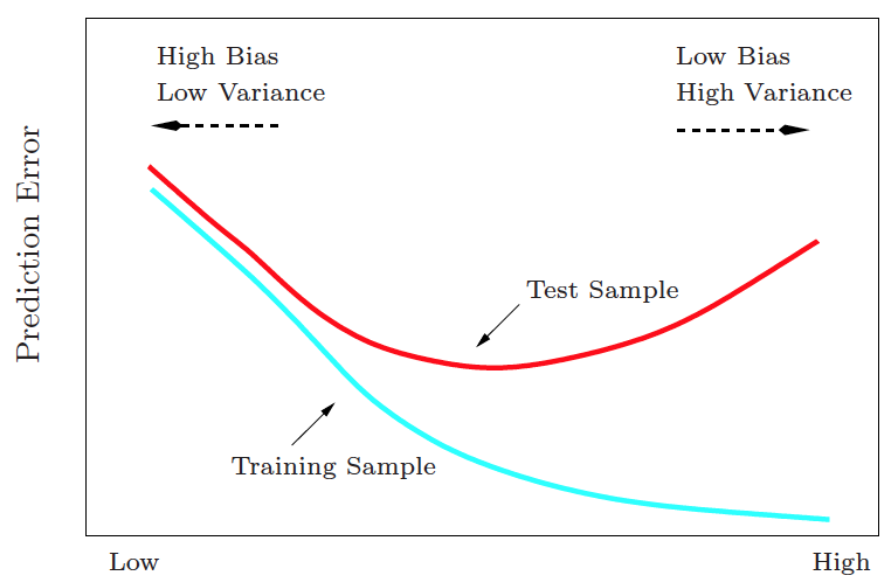
\includegraphics[width=0.75\textwidth]{bias_variance_tradeoff.png}
    \caption{Bias-Variance tradeoff: As model complexity increases, bias decreases and variance increases, leading to an optimal point of model complexity}
    \label{fig:bias_variance_tradeoff}
\end{figure}

The clearest example of overfitting is a interpolation of n data points with a polynomial of degree n-1. The model will have zero training error but will generalize poorly to new data.

\subsection{Training, validation and test sets}
\begin{itemize}
    \item \textbf{Training set} $T$: To fit the models
    \item \textbf{Validation set} $V$: To estimate prediction error for model selection  
\end{itemize}
If we are in a data-rich situation we can partition the data into three sets
\begin{enumerate}
    \item \textbf{Training set:} To fit the models
    \item \textbf{Validation set:} To estimate prediction error for model selection
    \item \textbf{Test set:} To estimate prediction error for the final model
\end{enumerate}

\subsection{K-fold cross validation}
\begin{enumerate}
    \item Define $K$ folds of the data
    \item For each fold $k$:
    \begin{enumerate}
        \item Train the model on the other $K-1$ folds
        \item Evaluate the model on fold $k$
    \end{enumerate}
\end{enumerate}
For example:
\begin{table}[H]
\centering
\begin{tabular}{|l|l|l|l|}
\hline
\textbf{Iteration} & \textbf{Training Folds} & \textbf{Validation Fold} & \textbf{Data Used for Validation} \\ \hline
Fold 1 & Folds 2, 3, 4, 5 (800 rows) & Fold 1 (200 rows) & Samples 1--200 \\ \hline
Fold 2 & Folds 1, 3, 4, 5 (800 rows) & Fold 2 (200 rows) & Samples 201--400 \\ \hline
Fold 3 & Folds 1, 2, 4, 5 (800 rows) & Fold 3 (200 rows) & Samples 401--600 \\ \hline
Fold 4 & Folds 1, 2, 3, 5 (800 rows) & Fold 4 (200 rows) & Samples 601--800 \\ \hline
Fold 5 & Folds 1, 2, 3, 4 (800 rows) & Fold 5 (200 rows) & Samples 801--1,000 \\ \hline
\end{tabular}
\end{table}

\subsection{Curse of dimensionality}
\begin{itemize}
    \item Easy problems in low-dimensional spaces can become difficult in high-dimensional spaces
    \item In high dimensions the distance between points increases
\end{itemize}

\subsection{Intuition of dimensionality}

\begin{itemize}
    \item There is no way to intuitively tell the need for dimensionality in higher dimensions
    \item Real data could have more than 1000 dimensions, but we can still find patterns in the data 
\end{itemize}
    
\subsection{Bias-variance trade off}
\begin{itemize}
    \item \textbf{Bias error}: The difference between the average prediction and the correct value
    \item \textbf{Variance error}: The variability of a model predicted datapoints
\end{itemize}
\begin{figure}[H]
    \centering
    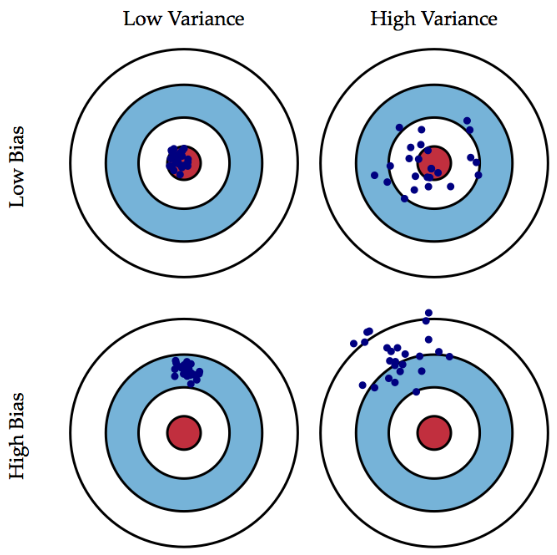
\includegraphics[width=0.5\textwidth]{bias_variance.png}
    \caption{Bias-Variance tradeoff: As model complexity increases, bias decreases and variance increases, leading to an optimal point of model complexity}
    \label{fig:bias_variance_tradeoff}
\end{figure}

\subsection{Bias-variance decomposition}
\begin{itemize}
    \item $f(\mathbf{x})$ -- true function
    \item $\hat{f}_{\mathcal{D}}$ -- prediction function 
\end{itemize}

Expected output value:
\[
E_{\mathcal{D}} \left[ \hat{f}_{\mathcal{D}}(\mathbf{x}) \right] \text{,\hspace{10pt} The average of models output over different sample sets}
\]

Mean squared error for estimating $f(\mathbf{x})$:
%===============================
% Fortsätt på sida 25 föreläsning 3
%===============================













\end{document}